\chapter{Aplicação da Abordagem}\label{case_study}

Este capítulo apresenta a aplicação da abordagem para especificação de sistemas orientados a aspectos em um sistema de gerenciamento de hotel.
A primeira seção apresenta a modelagem estrutural e comportamental dos interesses, especificando as características importantes da POA. Seguindo, são
apresentadas diferentes composições de interesses utilizando os aspectos especificados. Conclui-se com uma seção de discussão das vantagens da
abordagem e que destaca as principais características representadas.

\section{Modelagem do Sistema de Gerenciamento de Hotel}

Esta seção apresenta uma modelagem completa em alto nível de abstração de um sistema de gerenciamento de hotel, utilizando a abordagem proposta
por esta dissertação para realizar a separação e visualização de interesses. O exemplo é baseado no sistema para gerenciamento de hotel proposto por
Jacobson \cite{Jacobson:2004:ASD:1062430}. Este exemplo possibilita a modelagem de importantes funcionalidades de aspectos e foi utilizado para validar 
a abordagem de Jacobson. O exemplo de modelagem utiliza pontos de corte do tipo \textit{cflow} e \textit{cflowbelow}, que é um tipo de ponto de corte
com alto poder de expressividade da linguagem AspectJ, permitindo inserir comportamentos no fluxo de execução de um método. Também são especificados
avisos do tipo \textit{after} e \textit{before} e pontos de corte do tipo \textit{call}, \textit{throws} e \textit{execution}. A composição de
interesses com avisos do tipo \textit{around} (durante) também é tratada por este exemplo. Este tipo de aviso permite adicionar, remover ou
substituir um comportamento do sistema. Alguns pontos de corte são especificados com \textit{wildcards}, que permitem a captura de múltiplos pontos de
junção em uma única definição.

A modelagem deste exemplo contém diagramas estruturais e comportamentais, que utilizam as construções propostas pelo perfil UML para modelagem
de aspectos proposto por esta dissertação. Os diagramas de classes e de pacotes são utilizados para representar a estrutura dos aspectos. Para a
representação comportamental utilizam-se os diagramas de casos de uso, sequência e de máquina de estados. Os elementos presentes nos diagramas estruturais 
fornecem subsídios para a composição automática de diagramas de sequência, permitindo a troca de visões da dinâmica do sistema, visualizando
diferentes composições dos interesses núcleo com os interesses entrecortantes.

  \begin{figure}[!h]
	\centering
	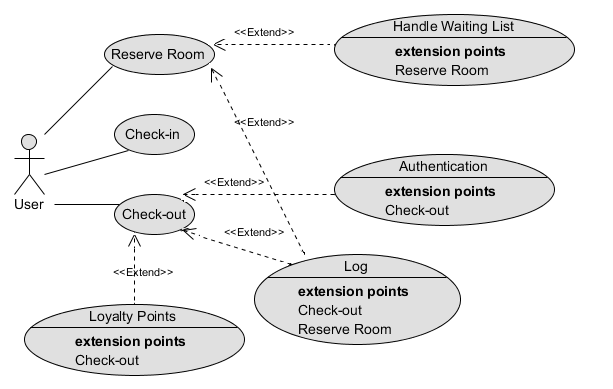
\includegraphics[scale=0.8]{img/case_study_use_cases.png}
	\caption{Diagrama de casos de uso do Sistema de Gerenciamento de Hotel.}\label{fig:case_study_use_cases}
  \end{figure}

A figura \ref{fig:case_study_use_cases} apresenta o diagrama de casos de uso do sistema de gerenciamento de hotel. Os casos de uso identificados em um sistema de 
gerenciamento de hotel são: reserva de quartos, tratamento de uma lista de espera para clientes, registro de mensagens, \textit{check-in} e
\textit{check-out} de clientes, acúmulo de pontos em um programa de fidelidade e autenticação. Os casos de uso de reserva de quartos,
\textit{check-in} e \textit{check-out} são interesses núcleo, pois são funcionalidades núcleo do sistema de gerenciamento de hotel. Os casos de uso de 
tratamento de lista de espera, registro de mensagens, acúmulo de pontos em um programa de fidelidade e autenticação são interesses entrecortantes,
pois estendem o comportamento das funcionalidades principais (dos interesses núcleo). Observa-se a presença do relacionamento \textit{<<Extend>>}
entre os casos de uso que representam interesses núcleo e os que representam interesses entrecortantes. Este relacionamento indica que o interesse
entrecortante adiciona algum comportamento no interesse núcleo. Na abordagem proposta, um caso de uso que representa um interesse entrecortante é
refinado em um ou mais pontos de corte (diagrama de máquina de estados) e um ou mais avisos (diagrama de sequência), que representam o comportamento
do aspecto. Os interesses núcleo são representados com o diagrama de sequência para representar seu comportamento. A parte estrutural de ambos
interesses é representada com o diagrama de classes e de pacotes.

O primeiro interesse representado é o de reserva de quartos, que permite que um cliente reserve um quarto no hotel. A modelagem de um interesse começa 
com a criação de um diagrama de classes que representa a sua estrutura. As classes e os aspectos que representam o interesse ficam agrupadas dentro de
um pacote da UML. Se o interesse for do tipo entrecortante, este pacote é marcado com o estereótipo \textit{CrosscuttingConcern}. No caso do interesse 
ser do tipo núcleo, o pacote não é estereotipado. O diagrama de classes da figura \ref{fig:case_study_structural_reserve_room} representa a estrutura
do interesse para reserva de quartos. A modelagem estrutural do interesse para reserva de quartos contém a classe \textit{Room} com o método
\textit{updateAvailability()} para atualizar a disponibilidade de um quarto. Este interesse também contém a classe \textit{ReserveRoomHandler} com o 
método \textit{makeReservation()}, responsável por realizar a reserva de um quarto.

  \begin{figure}[!h]
	\centering
	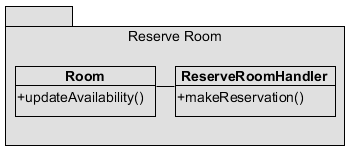
\includegraphics{img/case_study_structural_reserve_room.png}
	\caption{Modelagem estrutural: reserva de quarto}\label{fig:case_study_structural_reserve_room}
  \end{figure}

O segundo interesse modelado é o interesse entrecortante para registro de mensagens. Este interesse impacta vários componentes do sistema e é
marcado com o estereótipo \textit{CrosscuttingConcern}, para representar que o mesmo é entrecortante. A figura \ref{fig:case_study_structural_log}
apresenta a modelagem deste interesse. O interesse contém a classe \textit{Logger}, responsável por registrar as mensagens através do método
\textit{log()}. A classe \textit{Logger} é marcada com o estereótipo \textit{ClassExtension}, pois é uma nova classe no sistema. O método
\textit{log()} é estereotipado com \textit{Introduction}, pois é um método que está sendo inserido pelo interesse entrecortante para registro de mensagens. 
O aspecto \textit{LogAspect} é o aspecto que define os pontos de corte e avisos modelados nos diagramas de máquina de estados e nos digramas de
sequência. Existe uma associação entre o aspecto \textit{LogAspect} e a classe \textit{Logger}, pois o aspecto é o componente responsável por introduzir esta 
nova classe no sistema. Observa-se a presença do valor rotulado \textit{precedence} com o texto \textit{LogAspect, *}. Esta especificação define que o
aspecto para registro de mensagens tem precedência perante todos os outros aspectos do sistema (símbolo *), isto é, as mensagens deste aspecto serão
inseridas antes de outros aspectos no caso de um aviso conflitante do tipo antes. O mesmo vale para os outros tipos de aviso.

  \begin{figure}[!h]
	\centering
	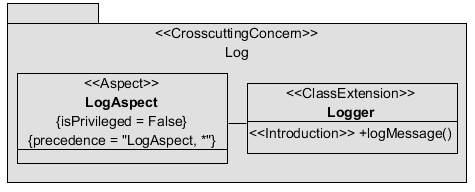
\includegraphics{img/case_study_structural_log.png}
	\caption{Modelagem estrutural: registro de mensagens}\label{fig:case_study_structural_log}
  \end{figure}
  
O interesse para controle de uma lista de espera de clientes é representado na modelagem da figura \ref{fig:case_study_structural_waiting_list}. O
pacote com as classes que representam o interesse também é marcado com o estereótipo \textit{CrosscuttingConcern}. O aspecto \textit{WaitingListAspect} está
associado com as classes \textit{WaitingListHandler}, \textit{Reservation} e \textit{WaitingList}. Essas três classes são extensões a classes do
sistema e estão estereotipadas com \textit{ClassExtension}. A classe \textit{WaitingListHandler} é a responsável pelo controle da lista de espera, com
o método \textit{putCustomerInWaitingList()}, que adiciona um cliente na lista de espera. A classe \textit{Reservation} contém um método para criar
uma reserva (\textit{createPendingReservation()}) e outro método para gerar um número para esta reserva (\textit{generatePendingReservationNumber()}).
Finalmente, a classe \textit{WaitingList} contém os métodos \textit{retrieveWaitingList()}, para obter a lista de espera, e o método
\textit{addPendingReservation()} para adicionar uma reserva de um cliente. Todos os métodos pertencentes a estas classes estão estereotipados com
\textit{Introduction}, pois são introduções estruturais ao sistema de gerenciamento de hotel.

  \begin{figure}[!h]
	\centering
	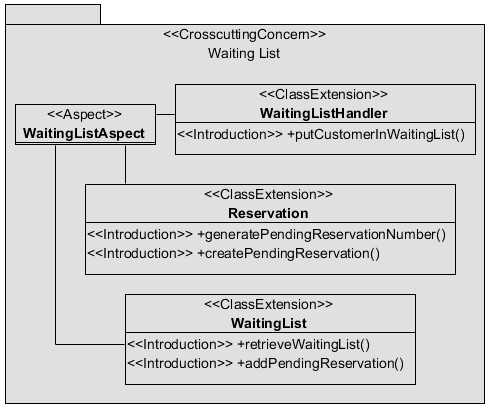
\includegraphics[scale=0.8]{img/case_study_structural_waiting_list.png}
	\caption{Modelagem estrutural: lista de espera}\label{fig:case_study_structural_waiting_list}
  \end{figure}
  
O interesse para \textit{check-in} de clientes permite realizar a entrada de clientes no hotel. A especificação estrutural deste interesse pode ser
visualizada na figura \ref{fig:case_study_structural_check_in}. Este interesse contém as classes \textit{CheckInHandler}, \textit{Room} e
\textit{Reservation}. A classe \textit{CheckInHandler} é responsável por iniciar o \textit{check-in} de um cliente. Ao iniciar o \textit{check-in}
chama-se o método \textit{queryReservation()} da classe \textit{Reservation} para verificar se existe alguma reserva para o cliente que está entrando
no hotel. Finalmente associa-se o cliente com um quarto através do método \textit{addCustomer()} da classe \textit{Room}. Este interesse não está
estereotipado, pois representa um interesse núcleo do sistema de gerenciamento de hotel.

  \begin{figure}[!h]
	\centering
	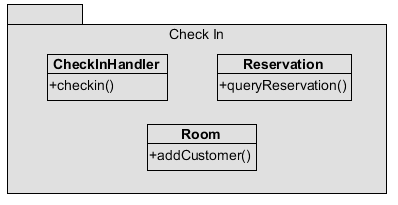
\includegraphics{img/case_study_structural_check_in.png}
	\caption{Modelagem estrutural: check-in de clientes}\label{fig:case_study_structural_check_in}
  \end{figure}

A especificação estrutural do interesse núcleo para \textit{check-out} de clientes pode ser visualizada na figura
\ref{fig:case_study_structural_check_out}. Este interesse contém a classe \textit{CheckOutHandler} que inicia a operação de \textit{check-out} através 
do método \textit{checkOut()}. A classe \textit{Payment} possui o método \textit{payBill()}, o qual permite realizar o pagamento de um quarto. O
usuário pode selecionar entre duas formas de pagamento: cartão ou dinheiro. A classe \textit{CardHandler} é responsável por tratar do pagamento em
cartão com os métodos \textit{checkCardInformation()} e \textit{performTransaction()} para realizar o pagamento. Se a opção de pagamento for dinheiro,
a responsabilidade é da classe \textit{MoneyHandler}, que realiza o pagamento através do método \textit{pay}. A classe \textit{Room} contém o método
\textit{removeCustomer()}, para remover um cliente da lista de hóspedes do hotel. As classes do modelo estrutural não estão estereotipadas, pois o
interesse de \textit{check-out} é um interesse núcleo do sistema.

  \begin{figure}[!h]
	\centering
	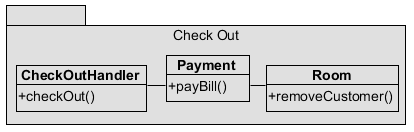
\includegraphics{img/case_study_structural_check_out.png}
	\caption{Modelagem estrutural: check-out de clientes}\label{fig:case_study_structural_check_out}
  \end{figure}

O interesse para acúmulo de pontos em um programa de fidelidade tem sua modelagem estrutural apresentada na figura
\ref{fig:case_study_structural_earn_points}. Este interesse é do tipo entrecortante, pois estende o sistema adicionando um novo requisito que
permite o acúmulo de pontos após o pagamento de um quarto. O pacote que representa o interesse é estereotipado com o estereótipo
\textit{CrosscuttingConcern}. A modelagem estrutural contém duas classes: \textit{LoyaltyPoints} e \textit{EarnPointsHandler}, marcadas com o
estereótipo \textit{ClassExtension}. A primeira classe contém o método \textit{addLoyaltyPoints()}, que adiciona pontos ao saldo do programa de
fidelidade de um determinado cliente. A classe \textit{EarnPointsHandler} contém o método \textit{earnCredits()}, o qual controla a operação de
obtenção de pontos após o pagamento. Finalmente, o aspecto \textit{EarnPointsAspect} contém o estereótipo \textit{Aspect}, e introduz as mudanças
estruturais propostas pelas classes deste interesse.

  \begin{figure}[!h]
	\centering
	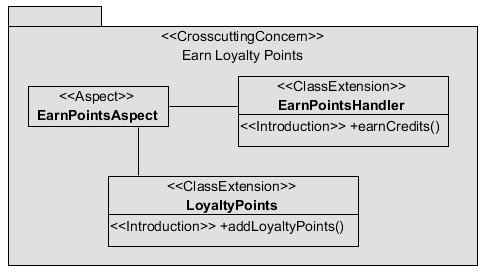
\includegraphics[scale=0.8]{img/case_study_structural_earn_points.png}
	\caption{Modelagem estrutural: acúmulo de pontos em programa de fidelidade}\label{fig:case_study_structural_earn_points}
  \end{figure}
  
A figura \ref{fig:case_study_structural_authentication} representa a estrutura do interesse para autenticação de usuários no sistema. A autenticação é
utilizado em algumas transações que exigem uma maior segurança. Este interesse é do tipo entrecortante (estereótipo \textit{CrosscuttingConcern}). O
diagrama de pacotes especificado contém a classe \textit{AuthHandler} com o método \textit{authenticate} e o aspecto \textit{AuthAspect} com o
estereótipo \textit{Aspect} e o método \textit{proceed()}. A chamada \textit{proceed} é uma diretiva da linguagem AspectJ que permite continuar a
execução do ponto de execução capturado por um ponto de corte. Este tipo de diretiva está associada a avisos do tipo \textit{around}, que permitem
substituir ou modificar inteiramente um ponto de execução de um sistema. 

  \begin{figure}[!h]
	\centering
	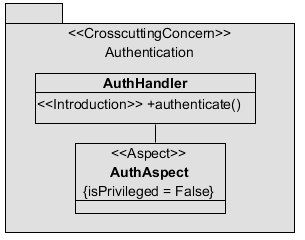
\includegraphics{img/case_study_structural_authentication.png}
	\caption{Modelagem estrutural: autenticação de usuários}\label{fig:case_study_structural_authentication}
  \end{figure}

Após a modelagem da estrutura dos interesses, deve-se modelar o comportamento dos mesmos. A especificação do comportamento de um interesse núcleo
envolve apenas o diagrama de sequência. Já os interesses entrecortantes devem ser modelados com um diagrama de máquina de estados para representar
seus pontos de corte e um diagrama de sequência para representar a execução do comportamento do aspecto. Os pontos de corte definem quais pontos do
sistema serão estendidos. O comportamento de um aspecto é representado pelos avisos associados ao mesmo. O diagrama de sequência que representa o
comportamento de um aspecto, também representa a conexão entre a satisfação de um ponto de corte com a execução das mensagens do aviso de um aspecto.

  \begin{figure}[!h]
	\centering
	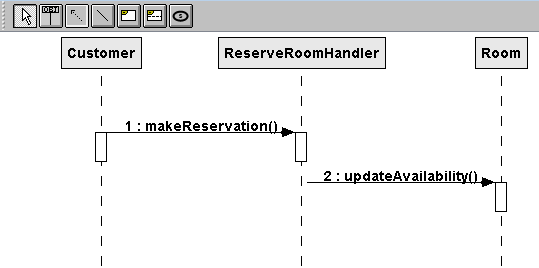
\includegraphics[scale=0.8]{img/case_study_behavioral_reserve_room.png}
	\caption{Diagrama de sequência: reserva de quarto}\label{fig:case_study_behavioral_reserve_room}
  \end{figure}

O primeiro diagrama de sequência é o que representa a troca de mensagens do interesse núcleo para reserva de quartos. O diagrama pode ser visualizado
na figura \ref{fig:case_study_behavioral_reserve_room}. Para realizar uma reserva de quarto, primeiramente realiza-se uma chamada ao método
\textit{makeReservation()} da classe \textit{ReserveRoomHandler}, que é responsável por iniciar a reserva. Após esta chamada, executa-se o método
para verificar se o quarto está disponível. Se o quarto não estiver disponível, uma exceção é lançada no método \textit{updateAvailability()}, caso
contrário, a reserva é realizada e o cliente recebe um código de confirmação. 

O interesse entrecortante para registro de mensagens contabiliza o número de requisições a um quarto. Para realizar este requisito, define-se um ponto
de corte que captura qualquer chamada (\textit{call}) a classes do tipo \textit{Room}. Este ponto de corte é modelado usando o diagrama de máquina de
estados da UML e pode ser visualizado na figura \ref{fig:case_study_behavioral_pointcut_log}.

  \begin{figure}
	\centering
	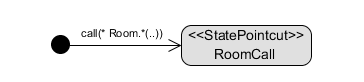
\includegraphics{img/case_study_behavioral_pointcut_log.png}
	\caption{Ponto de corte: registro de mensagens}\label{fig:case_study_behavioral_pointcut_log}
  \end{figure}

Com o ponto de corte especificado, cria-se o diagrama de sequência para representar a troca de mensagens entre objetos para realização do registro de
chamadas. O diagrama pode ser visualizado na figura \ref{fig:case_study_behavioral_log} e contém o aspecto \textit{LogAspect} associado a primeira linha 
de vida do diagrama. De acordo com a abordagem proposta, um aspecto no diagrama de sequência deve ter uma invariante de estado associada, a qual é o
gatilho para começar a executar a sequência de mensagens do diagrama. No exemplo em questão, a invariante de estado \textit{RoomCall} está associada 
ao aspecto \textit{LogAspect} e referencia o ponto de corte definido previamente no diagrama de máquina de estados. A semântica é que 
a sequência de mensagens só será executada quando o ponto de corte for satisfeito. A mensagem a ser executada é uma chamada ao método \textit{log()}
da classe \textit{Logger}. É importante observar o tipo de aviso, que é definido como um valor rotulado na invariante de estado. O valor rotulado 
não está sendo mostrado no diagrama de sequência por configuração de visualização, já que por padrão os valores rotulados não são exibidos. A
abordagem proposta suporta três tipos de aviso: antes, durante ou depois. Neste caso, o tipo de aviso é depois, o que significa que o comportamento de 
registro de mensagens somente executará após a chamada a qualquer método da classe \textit{Room}. O diagrama de sequência contém um fragmento
combinado do tipo opcional, o qual define que o registro de mensagens executará se a aplicação não estiver congelada. Uma aplicação está congelada quando 
está executando diretamente para o usuário e é considerada congelada no ambiente de desenvolvimento.
  
  \begin{figure}
	\centering
	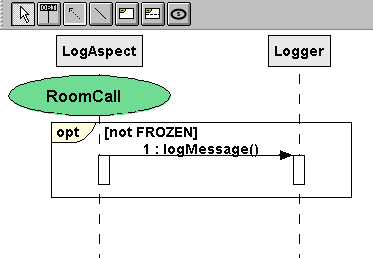
\includegraphics{img/case_study_behavioral_log.png}
	\caption{Aviso: registro de mensagens}\label{fig:case_study_behavioral_log}
  \end{figure}
  
Uma variação do interesse de registro de mensagens também é modelada. Esta variação não necessita que a aplicação esteja congelada para registro
das mensagens. O ponto de corte deste interesse entrecortante é modificado para capturar pontos de corte do tipo \textit{cflow} e \textit{cflowbelow}.
Estes tipos de ponto de corte capturam múltiplas chamadas após a chamada de um método. A figura \ref{fig:case_study_behavioral_pointcut_log_2} contém a 
especificação do ponto de corte para registro de mensagens. Este ponto de corte captura qualquer chamada de método dentro da execução do método
\textit{payBill()} da classe \textit{Payment}. Qualquer método que for chamado dentro deste método será capturado por este ponto de corte. 
O diagrama de sequência do interesse de registro de mensagens também é modificado, pois o mesmo não tem mais a restrição do sistema estar congelado
para executar o registro de mensagens. A figura \ref{fig:case_study_behavioral_log_2} apresenta o novo comportamento do interesse de registro de mensagens 
sem o fragmento combinado para verificar se o sistema está congelado.

  \begin{figure}[!h]
	\centering
	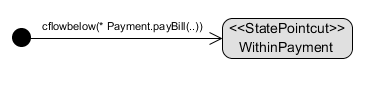
\includegraphics{img/case_study_behavioral_pointcut_log_2.png}
	\caption{Ponto de corte: registro de mensagens com fluxo de execução (cflow)}\label{fig:case_study_behavioral_pointcut_log_2}
  \end{figure}

  \begin{figure}[!h]
	\centering
	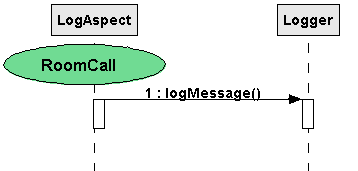
\includegraphics{img/case_study_behavioral_log_2.png}
	\caption{Ponto de corte: registro de mensagens sem restrições}\label{fig:case_study_behavioral_log_2}
  \end{figure}
  

O requisito para criação de uma lista de espera para clientes também é um interesse entrecortante. Este interesse adiciona um cliente a uma lista de
espera quando um quarto não está disponível. É necessário definir um ponto de corte que captura a tentativa de um cliente reservar um
quarto, mas o quarto está indisponível. A figura \ref{fig:case_study_behavioral_pointcut_waiting_list} representa um ponto de corte
para capturar as chamadas ao método \textit{updateAvailability()} da classe \textit{Room}, lançando a exceção \textit{NoRoomsAvailable}. Além da
definição de um ponto de corte, é necessário definir o comportamento de como um cliente é adicionado a lista de espera. O comportamento é modelado no
diagrama de sequência da figura \ref{fig:case_study_behavioral_waiting_list}. O diagrama tem o aspecto \textit{WaitingListAspect} associado a primeira 
linha de vida e uma sequência de mensagens para serem executadas quando o sistema lança uma exceção de quarto indisponível. Estas
mensagens são executadas depois do tratamento de exceção, pois o valor rotulado que define o tipo do aviso na invariante de estado é do tipo depois.

  \begin{figure}[tb]
	\centering
	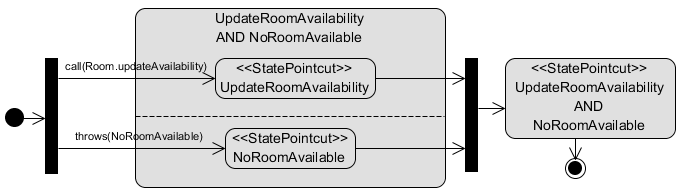
\includegraphics[scale=0.6]{img/case_study_behavioral_pointcut_waiting_list.png}
	\caption{Ponto de corte: controle de uma lista de espera}\label{fig:case_study_behavioral_pointcut_waiting_list}
  \end{figure}
 
 \begin{landscape}
  \begin{figure}[!h]
	\centering
	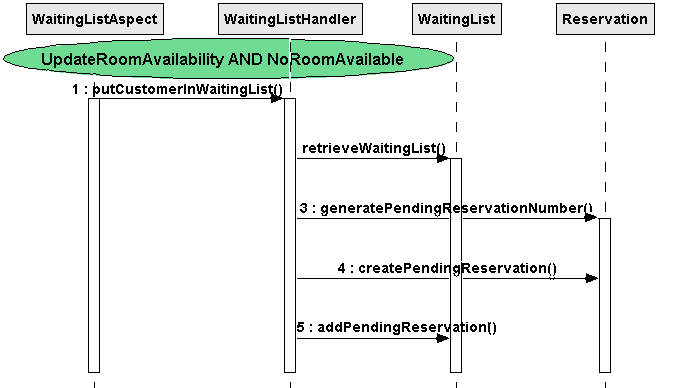
\includegraphics{img/case_study_behavioral_waiting_list.png}
	\caption{Aviso: controle de uma lista de espera}\label{fig:case_study_behavioral_waiting_list}
  \end{figure}
 \end{landscape}

O comportamento do interesse de \textit{check-in} de clientes pode ser visualizado na figura \ref{fig:case_study_behavioral_check_in}. A entrada de
clientes no hotel começa com a chamada do método \textit{checkIn()} da classe \textit{CheckInHandler}. Após a chamada deste método, é verificado se
existe alguma reserva para o cliente executando o método \textit{queryReservation()} da classe \textit{Reservation}. Com ou sem reserva o
\textit{check-in} procede chamando o método \textit{addCustomer()} da classe \textit{Room}. Este método associa o cliente ao quarto reservado ou
selecionado pelo mesmo. O interesse de \textit{check-in} de clientes é do tipo núcleo, por isso não contém nenhum aspecto no seu diagrama de
sequência.

  \begin{figure}[!h]
	\centering
	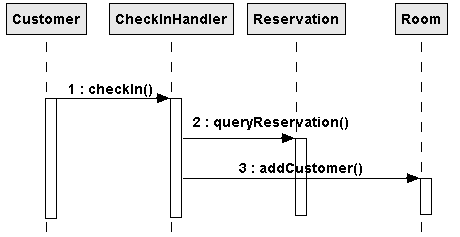
\includegraphics{img/case_study_behavioral_check_in.png}
	\caption{Diagrama de sequência: check-in de clientes}\label{fig:case_study_behavioral_check_in}
  \end{figure}

\begin{landscape}
  \begin{figure}[!h]
	\centering
	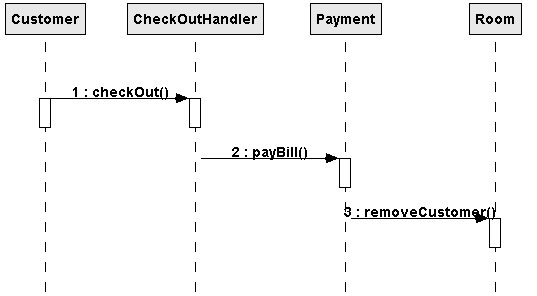
\includegraphics[scale=0.7]{img/case_study_behavioral_check_out.png}
	\caption{Diagrama de sequência: check-out de clientes}\label{fig:case_study_behavioral_check_out}
  \end{figure}
\end{landscape}

O diagrama de sequência que representa o comportamento do interesse para \textit{check-out} de clientes pode ser visualizado na figura
\ref{fig:case_study_behavioral_check_out}. A troca de mensagens do diagrama de sequência inicia quando o objeto \textit{CheckOutHandler} executa a
mensagem \textit{checkOut()}. Esta mensagem dispara a mensagem \textit{payBill()} para realizar o pagamento da conta do cliente. Neste momento o
cliente pode escolher o pagamento em dinheiro ou cartão. Se a opção for cartão, o método \textit{checkCardInformation()} é executado para
verificar as informações do cartão com a operadora. Se as informações estiverem de acordo executa-se o método \textit{performTransaction()} para
realizar a transação. Se a opção for dinheiro, executa-se o método \textit{pay()} da classe \textit{MoneyHandler}. Após o pagamento da conta, o
cliente é removido da lista de clientes ativos através do método \textit{removeCustomer()} da classe \textit{Room}.

A modelagem comportamental do interesse para acúmulo de pontos em um programa de fidelidade envolve a especificação de um ponto de corte e de um
aviso. O ponto de corte é especificado na figura \ref{fig:case_study_behavioral_pointcut_loyalty_points}. Este ponto de corte captura chamadas ao
método \textit{removeCustomer()} da classe \textit{Room}. O diagrama de sequência pode ser visualizado na figura
\ref{fig:case_study_behavioral_loyalty_points}. Este diagrama de sequência contém a invariante de estado \textit{BillPaid}, que está associada ao
aspecto \textit{EarnPointsAspect}. Esta invariante de estado contém o valor rotulado \textit{adviceType} com o valor \textit{after}. Isto significa que as
mensagens só serão executadas após a satisfação do estado \textit{BillPaid}. Após o disparo da invariante de estado, a classe
\textit{EarnPointsHandler} executa o método \textit{earnCredits()}. Este método dispara o método \textit{addLoyaltyPoints()} na classe
\textit{LoyalyPoints}, que adiciona pontos ao saldo de pontos do cliente no programa de fidelidade.

  \begin{figure}
	\centering
	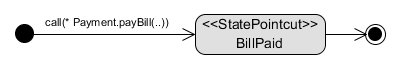
\includegraphics{img/case_study_behavioral_pointcut_authentication.png}
	\caption{Ponto de Corte: autenticação}\label{fig:case_study_behavioral_pointcut_authentication}
  \end{figure}

  \begin{figure}
	\centering
	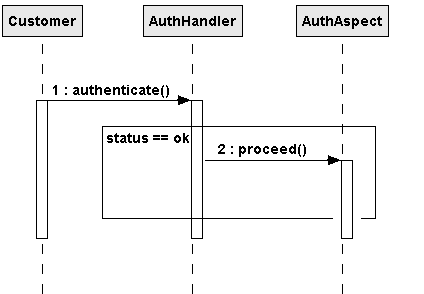
\includegraphics{img/case_study_behavioral_authentication.png}
	\caption{Aviso: autenticação}\label{fig:case_study_behavioral_authentication}
  \end{figure}

O último interesse entrecortante a ter seu comportamento especificado é o de autenticação. Este interesse é utilizado para dar mais segurança a
algumas transações do sistema de gerenciamento de hotel, como o pagamento da conta do usuário no momento de realizar o \textit{check-out} de um
cliente. A figura \ref{fig:case_study_behavioral_pointcut_authentication} apresenta o ponto de corte utilizado por este interesse para capturar em
quais partes do sistema a autenticação pode ser executada. Este ponto de corte captura chamadas ao método \textit{payBill()} da classe \textit{Payment}. 
O comportamento a ser adicionado pelo interesse de autenticação pode ser visualizado na figura
\ref{fig:case_study_behavioral_authentication}. Observa-se neste diagrama de sequência a chamada do método \textit{authenticate()} na classe 
\textit{AuthHandler}. Esta chamada inicia a autenticação de um usuário. Se o usuário for autenticado for sucesso, é executada a chamada
\textit{proceed()} no aspecto \textit{AuthAspect}. Esta chamada retorna a execução ao fluxo de execução original (do interesse núcleo sendo estendido
por este interesse entrecortante). Este tipo de substituição no fluxo de execução é adicionada por avisos do tipo \textit{around}. Este tipo de aviso
é representado pela diretiva \textit{proceed}.

  \begin{figure}[!h]
	\centering
	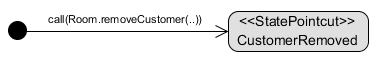
\includegraphics{img/case_study_behavioral_pointcut_loyalty_points.png}
	\caption{Ponto de corte: programa de fidelidade}\label{fig:case_study_behavioral_pointcut_loyalty_points}
  \end{figure}
  
  \begin{figure}[!h]
	\centering
	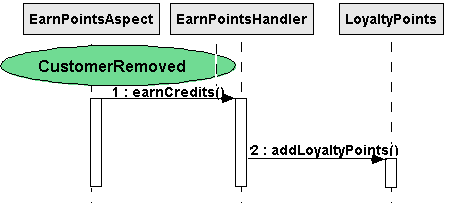
\includegraphics{img/case_study_behavioral_loyalty_points.png}
	\caption{Aviso: programa de fidelidade}\label{fig:case_study_behavioral_loyalty_points}
  \end{figure}

\begin{table*}[!h]
	\centering
	\begin{tabular}{ | c | c | c | c | c | c | c | c | c | c | }
		\hline
		 & Wildcard & Avisos & Introduções & Precedência & Pontos de Corte \\
		\hline
		 Fig & \ref{fig:case_study_behavioral_pointcut_log}, \ref{fig:case_study_behavioral_pointcut_authentication} 
		 &\ref{fig:case_study_behavioral_authentication}, \ref{fig:case_study_behavioral_loyalty_points},
		 \ref{fig:case_study_behavioral_pointcut_waiting_list}, \ref{fig:case_study_behavioral_pointcut_log} 
		 & \ref{fig:case_study_structural_authentication}, \ref{fig:case_study_structural_earn_points}, \ref{fig:case_study_structural_waiting_list},
		 \ref{fig:case_study_structural_log}
		 & \ref{fig:case_study_structural_log}
		 & \ref{fig:case_study_behavioral_pointcut_authentication}, \ref{fig:case_study_behavioral_pointcut_log},
		 \ref{fig:case_study_behavioral_pointcut_loyalty_points}, \ref{fig:case_study_behavioral_pointcut_waiting_list}, \ref{fig:case_study_behavioral_pointcut_log_2}
		 \\
		\hline
	\end{tabular}
	
	\caption{Características de aspectos representadas}
	\label{tab:aspects_characteristics}
\end{table*} 

A tabela \ref{tab:aspects_characteristics} apresenta as características de aspectos representadas na modelagem do sistema de
gerenciamento de hotel. Para cada característica, referenciam-se os diagramas (figuras) que modelam tal característica. A captura de múltiplos pontos
de junção em uma única chamada é representada nas figuras \ref{fig:case_study_behavioral_pointcut_log}
e \ref{fig:case_study_behavioral_pointcut_authentication}. O primeiro captura chamadas a qualquer método da classe \textit{Room}. Já o
segundo captura chamadas com qualquer número de parâmetros e qualquer tipo de retorno do método \textit{payBill()} da classe \textit{Payment}. Em relação aos avisos,
a figura \ref{fig:case_study_behavioral_authentication} representa avisos do tipo \textit{before} e \textit{around}. O aviso do tipo \textit{around}
permite executar comportamentos antes, durante ou depois de um dado comportamento. Neste caso, executa-se o comportamento de autenticação e depois
procede-se pra execução do fluxo de execução original. As figuras \ref{fig:case_study_behavioral_loyalty_points},
\ref{fig:case_study_behavioral_pointcut_waiting_list}, \ref{fig:case_study_behavioral_log} especificam avisos do tipo depois, isto é,
comportamentos que serão executados depois do fluxo original. Já as figuras \ref{fig:case_study_structural_authentication},
\ref{fig:case_study_structural_earn_points}, \ref{fig:case_study_structural_waiting_list} representam introduções e extensões a classes do modelo
estrutural núcleo do sistema de gerenciamento de hotel. As introduções são as construções que permitem modificar a estrutura de sistemas orientados a
aspectos. A ordem de precedência de aspectos é especificada pela figura \ref{fig:case_study_structural_log}, que estabelece que o interesse de
registro de mensagens tem precedência sobre os outros interesses. Finalmente, os diferentes tipos de ponto de corte e a composição entre os mesmos
também são atendidas pelos interesses do exemplo. A figura \ref{fig:case_study_behavioral_pointcut_waiting_list} apresenta a composição entre dois pontos de
corte, obtendo um ponto de corte composto de maneira automatizada. O ponto de corte do tipo \textit{cflowbelow} é representado na figura
\ref{fig:case_study_behavioral_pointcut_log_2} e captura chamadas no fluxo de execução de um método. As figuras
\ref{fig:case_study_behavioral_pointcut_log}, \ref{fig:case_study_behavioral_pointcut_authentication} e
\ref{fig:case_study_behavioral_pointcut_loyalty_points} especificam pontos de corte do tipo \textit{call}. Estes tipos de ponto de corte capturam
chamadas a métodos de um sistema.

\section{Composição e Visualização de Interesses}

Depois da especificação estrutural e comportamental dos interesses núcleo e entrecortantes, o desenvolvedor pode intercambiar as visões do sistema,
selecionando quais interesses deseja visualizar em um mesmo diagrama. A ferramenta SEA/Aspect permite a seleção de um ou mais modelos para serem
compostos. A ferramenta realiza a composição estrutural (se houver introduções) dos diagramas de classe e comportamental dos diagramas de sequência.

A primeira composição envolve três interesses do sistema:

\begin{itemize}
  \item \textbf{Reserva de Quartos:} Um cliente pode reservar um quarto, se o mesmo estiver disponível.
  \item \textbf{Registro de Mensagens:} O sistema registra as mensagens executadas em determinados componentes.
  \item \textbf{Lista de Espera:} Um cliente pode ser colocado em uma lista de espera quando um quarto não estiver disponível para reserva imediata.
\end{itemize}

A figura \ref{fig:case_study_compound_2_structural} apresenta a composição estrutural deste exemplo, contendo as diferentes classes compostas, com
introduções de métodos, atributos e relacionamentos. Observa-se a adição das classes \textit{Logger} com o método \textit{logMessage()},
\textit{WaitingListHandler} com o método \textit{putCustomerInWaitingList()}, \textit{WaitingList} com os métodos \textit{retrieveWaitingList} e
\textit{generatePendingReservationNumber()} e \textit{Reservation} com os métodos \textit{createPendingReservation()} e
\textit{addPendingReservation()}. Alem da adição de classes e métodos, a composição estrutural também adicionou relacionamentos entre as classes
\textit{ReserveRoomHandler} e \textit{Logger} e entre \textit{ReserveRoomHandler} e \textit{WaitingListHandler}. Estes relacionamentos são adicionados
entre as classes que representam o interesse núcleo e as que representam os interesses entrecortantes.

A composição do comportamento destes interesses pode ser visualizada na figura \ref{fig:case_study_compound_2}, com os interesses
para reserva de quarto, registro de mensagens e tratamento da lista de espera. Atribui-se uma cor diferente a cada interesse do modelo composto. 
A mensagem do interesse de registro de mensagens (\textit{logMessage()}) está com o fundo vermelho. Já as mensagens do interesse para controle de uma
lista de espera (\textit{putCustomerInWaitingList(), retrieveWaitingList(), generatePendingReservationNumber(), createPendingReservation() e addPendingReservation()})
estão com o fundo verde. As mensagens do interesse de reserva de quarto estão com o fundo branco. O diagrama composto exibe um seletor de modelos na
parte de baixo da imagem, o qual permite a troca dos modelos que estão sendo compostos. A composição comportamental de interesses é realizada
baseando-se nos diagramas de sequência e de máquina de estados dos interesses núcleo e entrecortantes. A mensagem \textit{logMessage()} foi adicionada
depois das mensagens do interesse núcleo de reserva de quartos, pois o diagrama de sequência (\ref{fig:case_study_behavioral_log}) que representa o aspecto de
registro de mensagens contém um aviso do tipo \textit{after} e o ponto de corte (\ref{fig:case_study_behavioral_pointcut_log}) do interesse de registro de mensagens 
captura chamadas a qualquer método da classe \textit{Room}. As mensagens do interesse entrecortante de lista de espera também foram adicionadas depois
das mensagens de reserva de quarto, pois o aviso no diagrama de sequência (\ref{fig:case_study_behavioral_waiting_list}) de lista de espera também é 
do tipo \textit{after} e o ponto de corte (\ref{fig:case_study_behavioral_pointcut_waiting_list} captura chamadas ao método \textit{updateAvailability()} da 
classe \textit{Room}. É importante observar que o interesse para registro de mensagens tem precedência perante o interesse para controle de uma lista
de espera, por isso a mensagem \textit{log()} foi introduzida antes das mensagens do interesse de lista de espera no diagrama de sequência composto. 
A ordem de precedência é definida pelo valor rotulado \textit{precedence}, configurado ao definir a estrutura do interesse de registo de mensagens na figura
\ref{fig:case_study_structural_log}.

  \begin{figure}[!h]
	\centering
	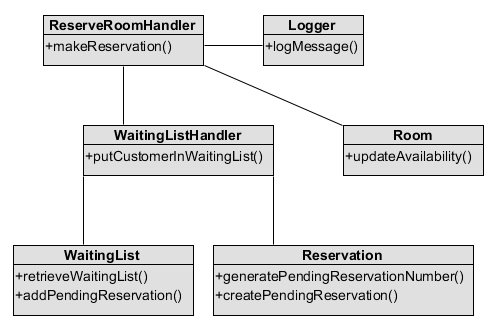
\includegraphics[scale=0.8]{img/case_study_compound_2_structural.png}
	\caption{Modelo Estrutural: reserva de quarto composto com registro de mensagens e controle de lista de espera}\label{fig:case_study_compound_2_structural}
  \end{figure}
  
\begin{landscape}
  \begin{figure*}
	\centering
	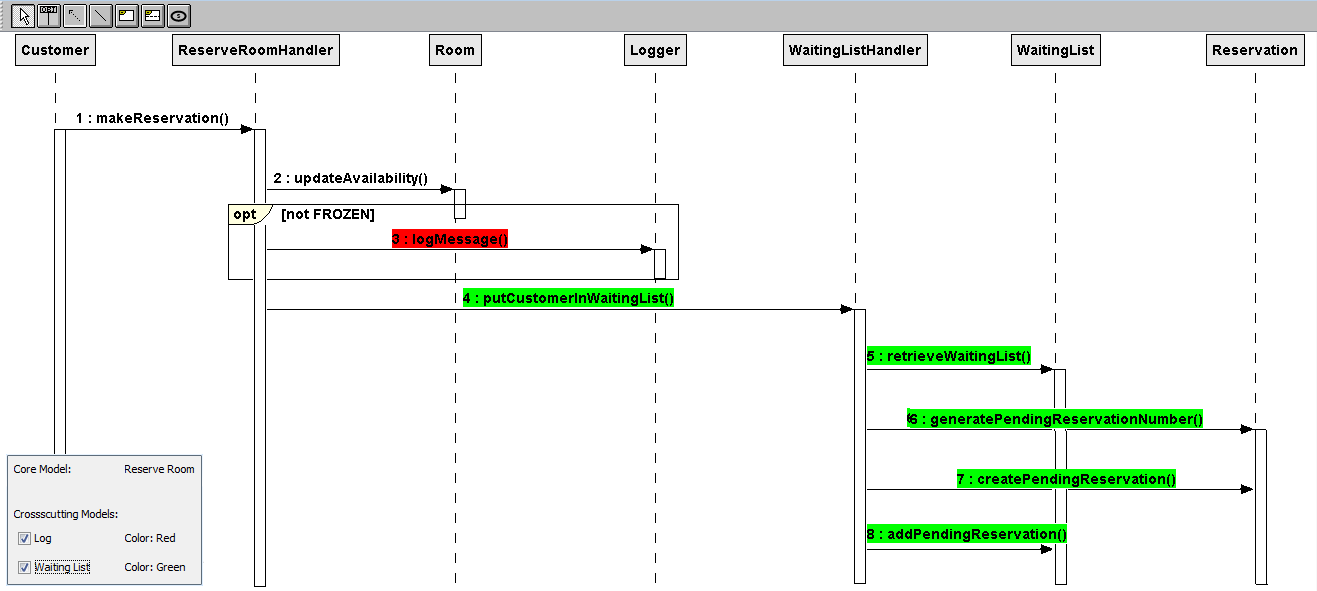
\includegraphics[scale=0.5]{img/case_study_compound_2.png}
	\caption{Modelo Comportamental: reserva de quarto composto com registro de mensagens e controle de lista de espera}\label{fig:case_study_compound_2}
  \end{figure*}
\end{landscape}

É possível realizar diferentes configurações de interesses utilizando a ferramenta SEA/Aspect. A figura \ref{fig:case_study_compound_1_structural}
apresenta a composição estrutural apenas dos interesses para reserva de quarto e registro de mensagens, sem o interesse de adição de clientes em uma lista de
espera quando um quarto não estiver disponível. O usuário pode realizar estas modificações dinamicamente, obtendo o resultado rapidamente. A
composição comportamental desta configuração também pode ser visualizada na figura \ref{fig:case_study_compound_1}

  \begin{figure}[!h]
	\centering
	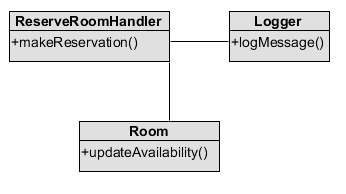
\includegraphics{img/case_study_compound_1_structural.png}
	\caption{Modelo Estrutural: reserva de quarto composto com registro de mensagens}\label{fig:case_study_compound_1_structural}
  \end{figure}

  \begin{figure}[!h]
	\centering
	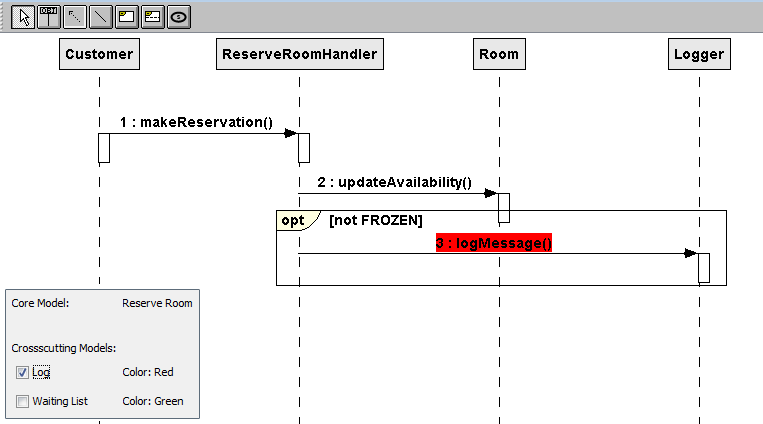
\includegraphics[scale=0.6]{img/case_study_compound_1.png}
	\caption{Modelo Comportamental: reserva de quarto composto com registro de mensagens}\label{fig:case_study_compound_1}
  \end{figure}

A segunda composição a ser executada tem uma maior complexidade, pois envolve avisos do tipo \textit{before}, \textit{around} e \textit{after} em uma
mesma configuração de interesses. Esta composição envolve quatro interesses do sistema:

\begin{itemize}
  \item \textbf{Check-out:} A ação executada quando um cliente sai do hotel liberando um quarto.
  \item \textbf{Acúmulo de Pontos em um Programa de Fidelidade:} Um cliente pode acumular pontos em um programa de fidelidade ao realizar o pagamento
  da sua conta.
  \item \textbf{Autenticação:} Algumas transações devem ser autenticadas pelo sistema.
  \item \textbf{Registro de Mensagens (sem restrições):} O sistema registra as mensagens executadas em determinados componentes.
\end{itemize}

A figura \ref{fig:case_study_2_compound_structural} apresenta a composição estrutural dos interesses para \textit{check-out} de clientes, acúmulo
de pontos em um programa de fidelidade, autenticação de usuários e registro de mensagens. Observa-se a adição das classes \textit{AuthHandler} do
interesse entrecortante de autenticação, \textit{LoyaltyPoints} e \textit{EarnPointsHandler} do interesse entrecortante de acúmulo de pontos em um
programa de fidelidade e \textit{Logger} do interesse entrecortante para registro de mensagens. As outras classes são do interesse núcleo para
\textit{check-out} de clientes. A ferramenta de composição estrutural também adiciona os relacionamentos entre as classes dos interesses núcleo com
as classes dos interesses entrecortantes.
  
A figura \ref{fig:case_study_2_compound} apresenta a composição comportamental dos interesses. Os diagramas de sequência que representam os aspectos
dos interesses entrecortantes contém avisos dos três tipos possíveis na linguagem AspectJ: \textit{before}, \textit{after} e \textit{around}. As
mensagens do interesse de \textit{check-out} de clientes estão com o fundo verde. O interesse de autenticação contém mensagens diferenciadas com
a cor rosa. Já as mensagens do interesse de registro de mensagens estão coloridas em amarelo. O interesse de acúmulo de pontos em um programa de
fidelidade está com a cor azul. Observa-se nesta composição a inserção da mensagem \textit{authenticate()} antes (\textit{before}) da mensagem
\textit{payBill()}. Esta mensagem foi adicionada nesta posição devido ao ponto de corte (\ref{fig:case_study_behavioral_pointcut_authentication}) e
aviso (\ref{fig:case_study_behavioral_authentication}) do tipo \textit{around} do interesse entrecortante de autenticação. O comportamento do interesse 
entrecortante de autenticação só continua o fluxo de execução se a autenticação for bem sucedida (através da chamada \textit{proceed()}. No diagrama
composto, este comportamento pode ser visualizado através do fragmento combinado \textit{status == ok}. Um pagamento só será realizado se o usuário estiver 
autenticado. Outro comportamento adicionado por um aspecto é o de registro de mensagens no fluxo de execução do método \textit{payBill()}. Este
comportamento é definido pelo ponto de corte \textit{cflowbelow} (\ref{fig:case_study_behavioral_pointcut_log_2}) e pelo aviso (\ref{fig:case_study_behavioral_log_2}) 
do tipo \textit{after} definido pelo interesse de registro de mensagens. O último comportamento adicionado é o de ganho de pontos em um programa de
fidelidade após o pagamento de uma conta. Este comportamento é adicionado após o método \textit{removeCustomer()} devido a definição do ponto de corte
que captura chamadas ao método \textit{removeCustomer()} da classe \textit{Room} e devido ao aviso
(\ref{fig:case_study_behavioral_pointcut_loyalty_points}) que executa as mensagens para acúmulo de pontos no programa de fidelidade após
(\textit{after}) a captura do ponto de corte.

  \begin{figure}[!h]
	\centering
	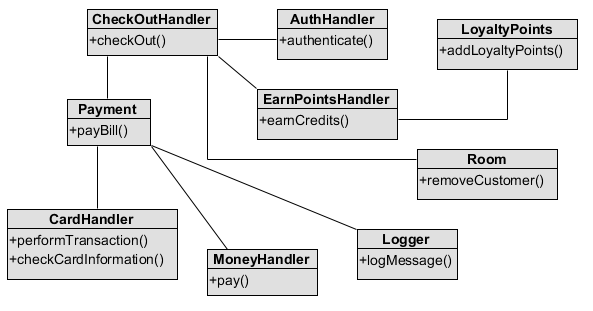
\includegraphics[scale=0.7]{img/case_study_2_compound_structural.png}
	\caption{Modelo Estrutural: check-out de clientes composto com registro de mensagens, autenticação de usuários e programa de
	fidelidade}\label{fig:case_study_2_compound_structural}
  \end{figure}

  \begin{landscape}
  \begin{figure*}[tb]
	\centering
	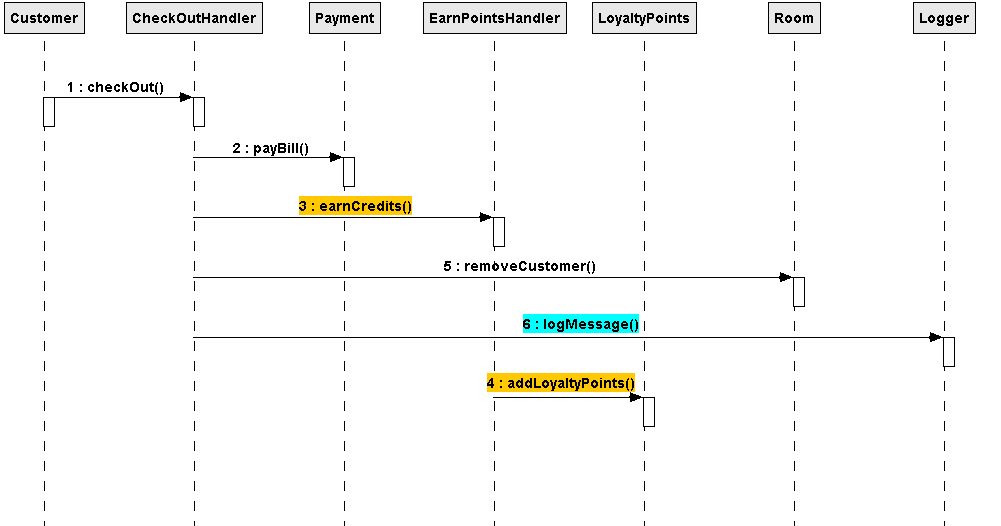
\includegraphics[scale=0.5]{img/case_study_2_compound.png}
	\caption{Modelo Comportamental: check-out de clientes composto com registro de mensagens, autenticação de usuários e programa de
	fidelidade}\label{fig:case_study_2_compound}
  \end{figure*}
\end{landscape}

Com a ferramenta SEA/Aspect o desenvolvedor pode modificar dinamicamente quais interesses estão sendo visualizados no modelo composto. Assim, o
desenvolvedor poderia realizar uma nova configuração de interesses, adicionando o interesse de autenticação para todas chamadas do sistema, por
exemplo. Esta mudança não demanda nenhum esforço do desenvolvedor, pois a ferramenta realiza automaticamente a nova composição de modelos. A
ferramenta permite realizar diferentes composições de interesses, alternando as visões do sistema.

\section{Discussão}

A aplicação da abordagem em um exemplo prático mostra como a proposta para especificação e composição de aspectos facilita a compreensão de
sistemas orientados a aspectos, permitindo a alternância de visões, visualizando somente os interesses núcleo ou uma composição entre interesses núcleo e entrecortantes, 
sem esforço do desenvolvedor. Os modelos compostos mostram o efeito dos aspectos em um sistema, com cada aspecto diferenciado por uma única cor que o
representa. A ferramenta SEA/Aspect permite a separação de interesses nas primeiras fases de desenvolvimento, o que é um dos objetivos das abordagens para modelagem
de sistemas orientados a aspectos. É importante destacar também que esta modelagem é a primeira que representa pontos de corte de fluxos de execução
(\textit{cflow} e \textit{cflowbelow}) e também permite realizar a composição de avisos do tipo \textit{around}.
